\documentclass{article}

% Language setting
% Replace `english` with e.g. `spanish` to change the document language
\usepackage[english]{babel}

% Set page size and margins
% Replace `letterpaper` with `a4paper` for UK/EU standard size
\usepackage[letterpaper,top=2cm,bottom=2cm,left=3cm,right=3cm,marginparwidth=1.75cm]{geometry}

\renewcommand{\thesubsection}{\arabic{subsection})}
% Useful packages
\usepackage{booktabs}
\usepackage{amsmath}
\usepackage{float}
\usepackage{graphicx}
\usepackage[T1]{fontenc} % Corrected encoding issue
\usepackage[colorlinks=true, allcolors=blue]{hyperref}

\title{Raport zaliczeniowy \\
Analiza cen zawodników angielskiej Premier League w zależności od ich statystyk}
\author{Maksym Selishchev \\
Informatyka Stosowana \\
Politechnika Wrocławska \\
MSiD Lab 9:15}

\begin{document}
\maketitle

\section{Opis problemu}

Problemem wybranym do badań jest przewidywanie cen zawodników angielskiej Premier League w zależności od różnych czynników. Analiza zbioru może wykazać przybliżoną cenę zawodnika na podstawie jego statystyk, drużyny, wieku itd. Celem projektu jest zbadanie zależności od dostępnych parametrów:
\begin{itemize}
    \item Liczba zagranych minut w sezonie
    \item Drużyna
    \item Wiek
    \item Liczba bramek i asyst
    \item Pozycja
    \item Kraj pochodzenia
\end{itemize}
oraz stworzenie modelu estymującego cenę na podstawie wybranych danych.




\section{Zbiór danych i jego przetwarzanie}

\subsection{Zbiór danych}
W pracy zostały wykonane 4 zbiory danych:
\begin{enumerate}
    \item Zbiór 1 "Dane zawodników i ich cena w konkretnym terminie"  pozyskany z Kaggle. Zawiera dane o id zawodnika oraz jego cenę za ostatnie 25 lat.
    \item Zbiór 2 "Dane osobiste zawodników" posiada id, imię, nazwisko, ligę, kraj pochodzenia, miasto urodzeina i wiele innych informacji zawodnika. Faktycznie zbiór jest powiązany ze zbiorem 1 po id. Też pozyskany z Kaggle.
    \item Zbiór 3 "Statystyka zawodników angielskiej Premier Ligue w sezonie 2018/2019". Zawiera dane statystyczne graczy takie jak liczba minut zagranych w sezonie, strzałów, bramek, asyst i wiele innych. Pozyskany z footystats.
    \item Zbiór 4 tabela wynników drużyn w angielskiej Premier Ligue w sezonie 2018/2019 zawiera posortowane według liczby punktów drużyny, liczbę punktów oraz cenę całej drużyny. Pozyskany z Eurosport.com 
\end{enumerate}
\subsection{Przetwarzanie danych do analizy}

\begin{enumerate}
    \item W zbiorze 1 zostały tylko kolumny reprezentujące id zawodnika oraz jego cenę w terminach '2019-04-01'-'2019-07-01'.
    \begin{table}[htb]
        \centering
        \caption{Cena zawodników}
        \label{tab:vehicle_data_1}
        \begin{tabular}{cc}
        \toprule
        Id & Cena  \\
        \midrule
        321 & 80000000  \\
        204 & 12000000  \\
        \bottomrule
        \end{tabular}
    \end{table}

    \item W zbiorze 2 zostały tylko kolumny reprezentujące id zawodnika oraz jego imię i nazwisko. Zbiór został połączony ze zbiorem 1 po id zawodnika

   \begin{table}[htb]
        \centering
        \caption{Dane zawodników}
        \label{tab:vehicle_data_1}
        \begin{tabular}{ccc}
        \toprule
        Id & Cena & Imię i nazwisko  \\
        \midrule
        321 & 80000000 & Cristiano Ronaldo \\
        204 & 12000000 & Lionel Messi  \\
        \bottomrule
        \end{tabular}
    \end{table}    
    
    \item W zbiorze 3 zostały tylko kolumny reprezentujące podstawowe statystyki zawodnika w sezonie i też został połączony z dwoma zbiorami wyżej. 
    
   \begin{table}[H]
    \centering
    \caption{Statystyka zawodników}
    \label{tab:vehicle_data_1}
    \begin{tabular}{cccccc}
    \toprule
    Id & Cena & Imię i nazwisko & Liczba zagranych minut & Liczba bramek & Klub  \\
    \midrule
    321 & 80000000 & Cristiano Ronaldo & 1234 & 34 & Manchester United\\
    204 & 12000000 & Lionel Messi & 5124 & 40 & Chelsea\\
    \midrule
    \multicolumn{2}{c}{Pozycja} & Kraj pochodzenia & Liczba asyst & Wiek & \\
    \midrule
    \multicolumn{2}{c}{Napastnik} & Portugalia & 3 & 38 & \\
    \multicolumn{2}{c}{Napastnik} & Argentyna & 9 & 35 & \\
    \bottomrule
    \end{tabular}
\end{table}


    \item Do zbioru 4 ręcznie była dodana cena klubu i zostały tylko nazwy, punkty i cena

    \begin{table}[H]
        \centering
        \caption{Tabela klubów}
        \label{tab:vehicle_data_1}
        \begin{tabular}{ccc}
        \toprule
        Klub & Punkty & Cena \\
        \midrule
        Machester United & 32 & 10000000\\
        Manchester City & 54 & 20000000\\
        \bottomrule
        \end{tabular}
    \end{table}
 
\end{enumerate}

Zbiór 4 też został połaczony z 3 zbiorami wyżej po połączeniu okazało się, że tylko 354/447 zawodników mają przypisane punkty i ceny klubów, dla wypełnienia pustych komórek była wykorzystana losowa liczba między średnią z kolumny +- 30 procent.




\section{Eksperymenty}

\textbf{Analiza zależności}


\begin{figure}[H]
    \centering
        \begin{minipage}{0.5\textwidth} 
        \centering Zależność ceny od minut zagranych w sezonie :
    \end{minipage}
    \begin{minipage}{1\textwidth} 
        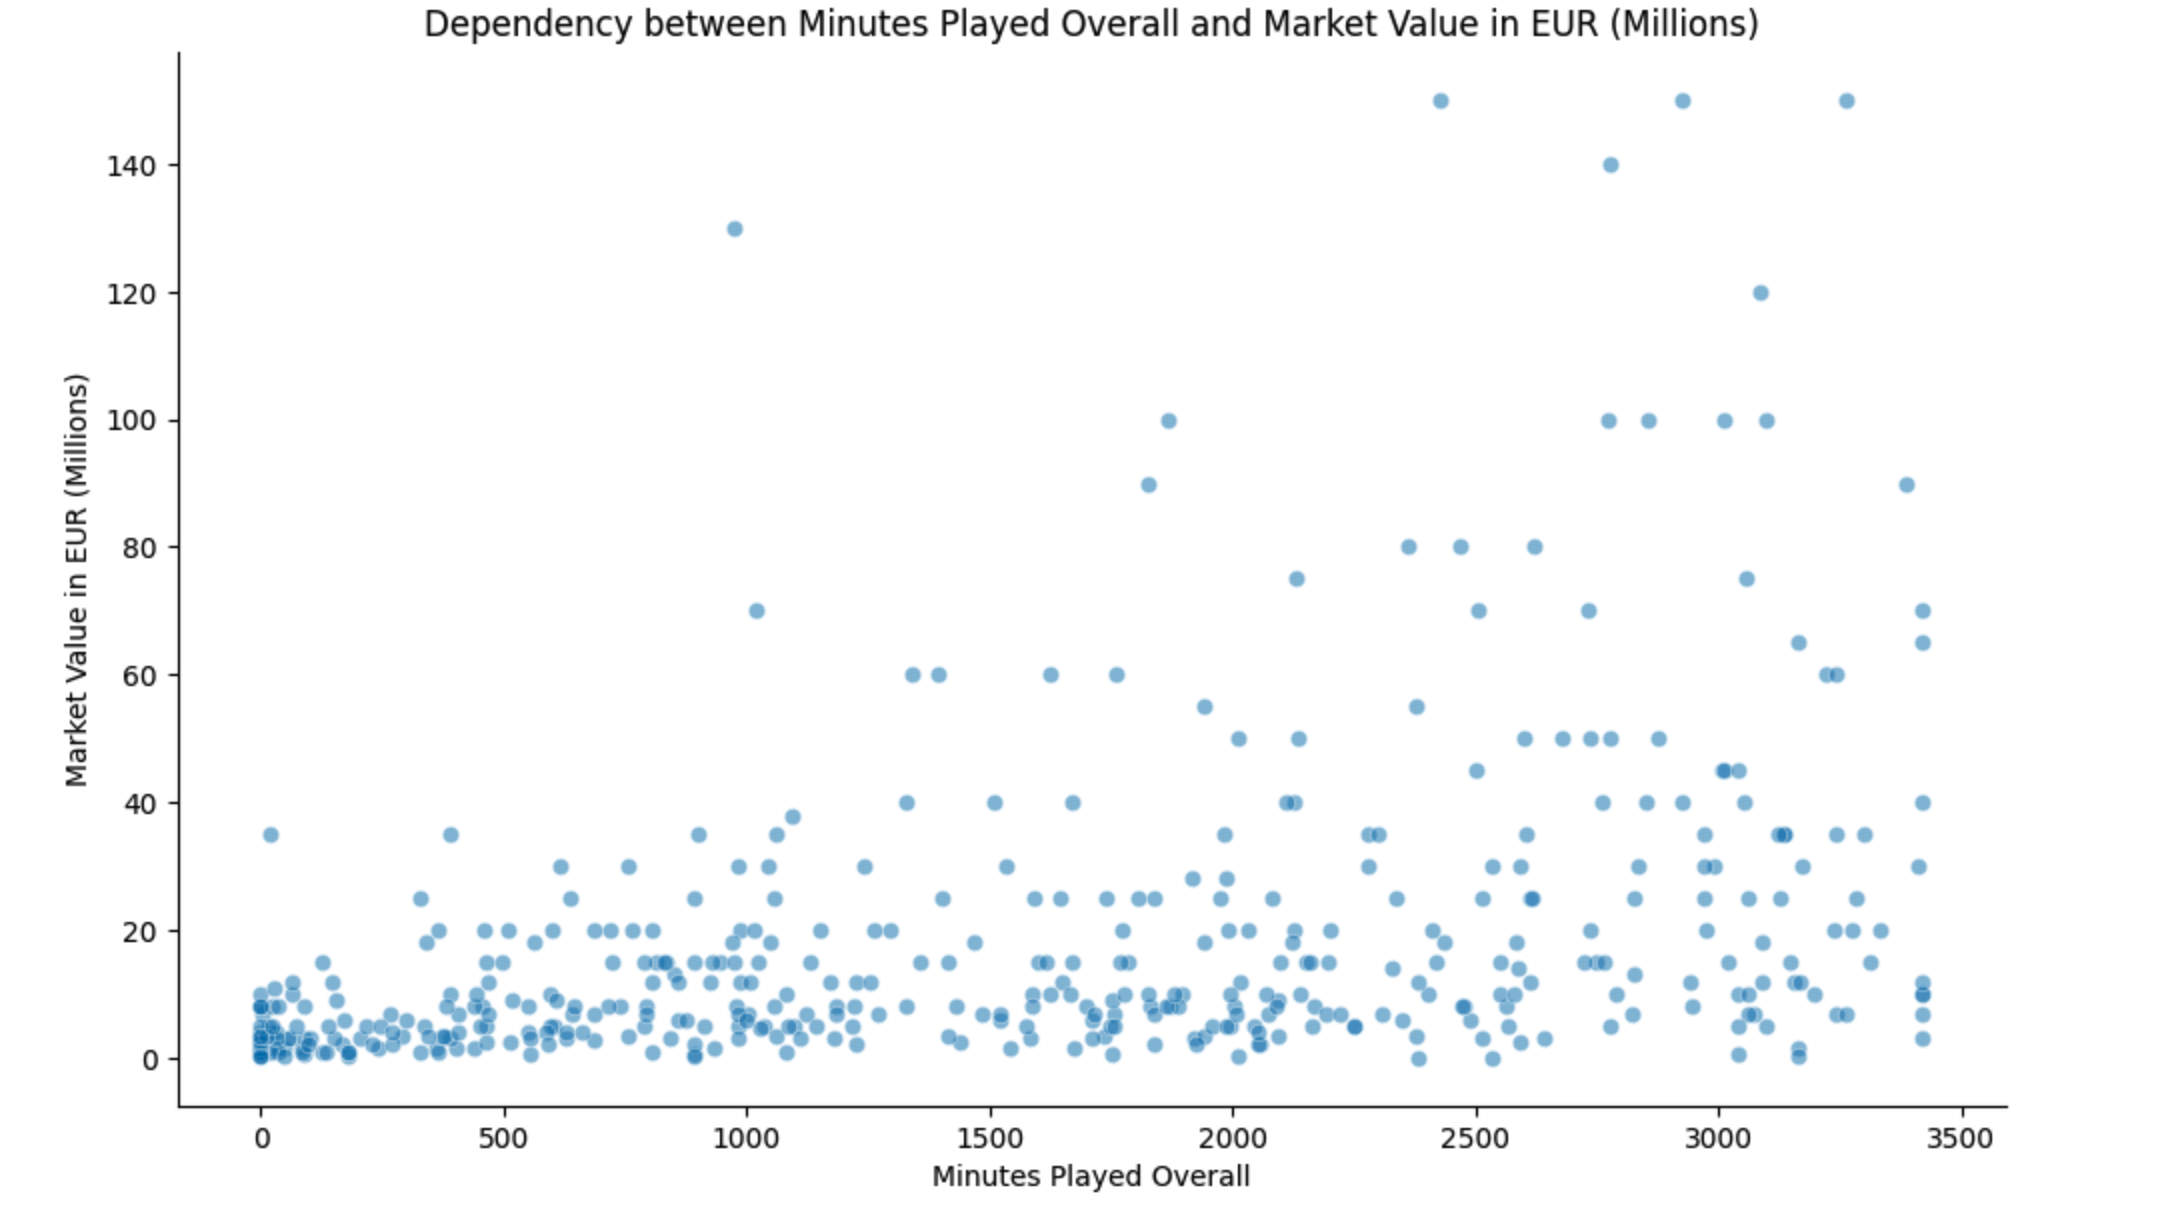
\includegraphics[width=\linewidth]{minutes.png} 
        \label{fig:zdjecie}
    \end{minipage}
    \hfill 

\end{figure}

\begin{figure}[H]
    \centering
        \begin{minipage}{0.5\textwidth} 
        \centering Zależność ceny od strzelonych bramek :
    \end{minipage}
    \begin{minipage}{1\textwidth} 
        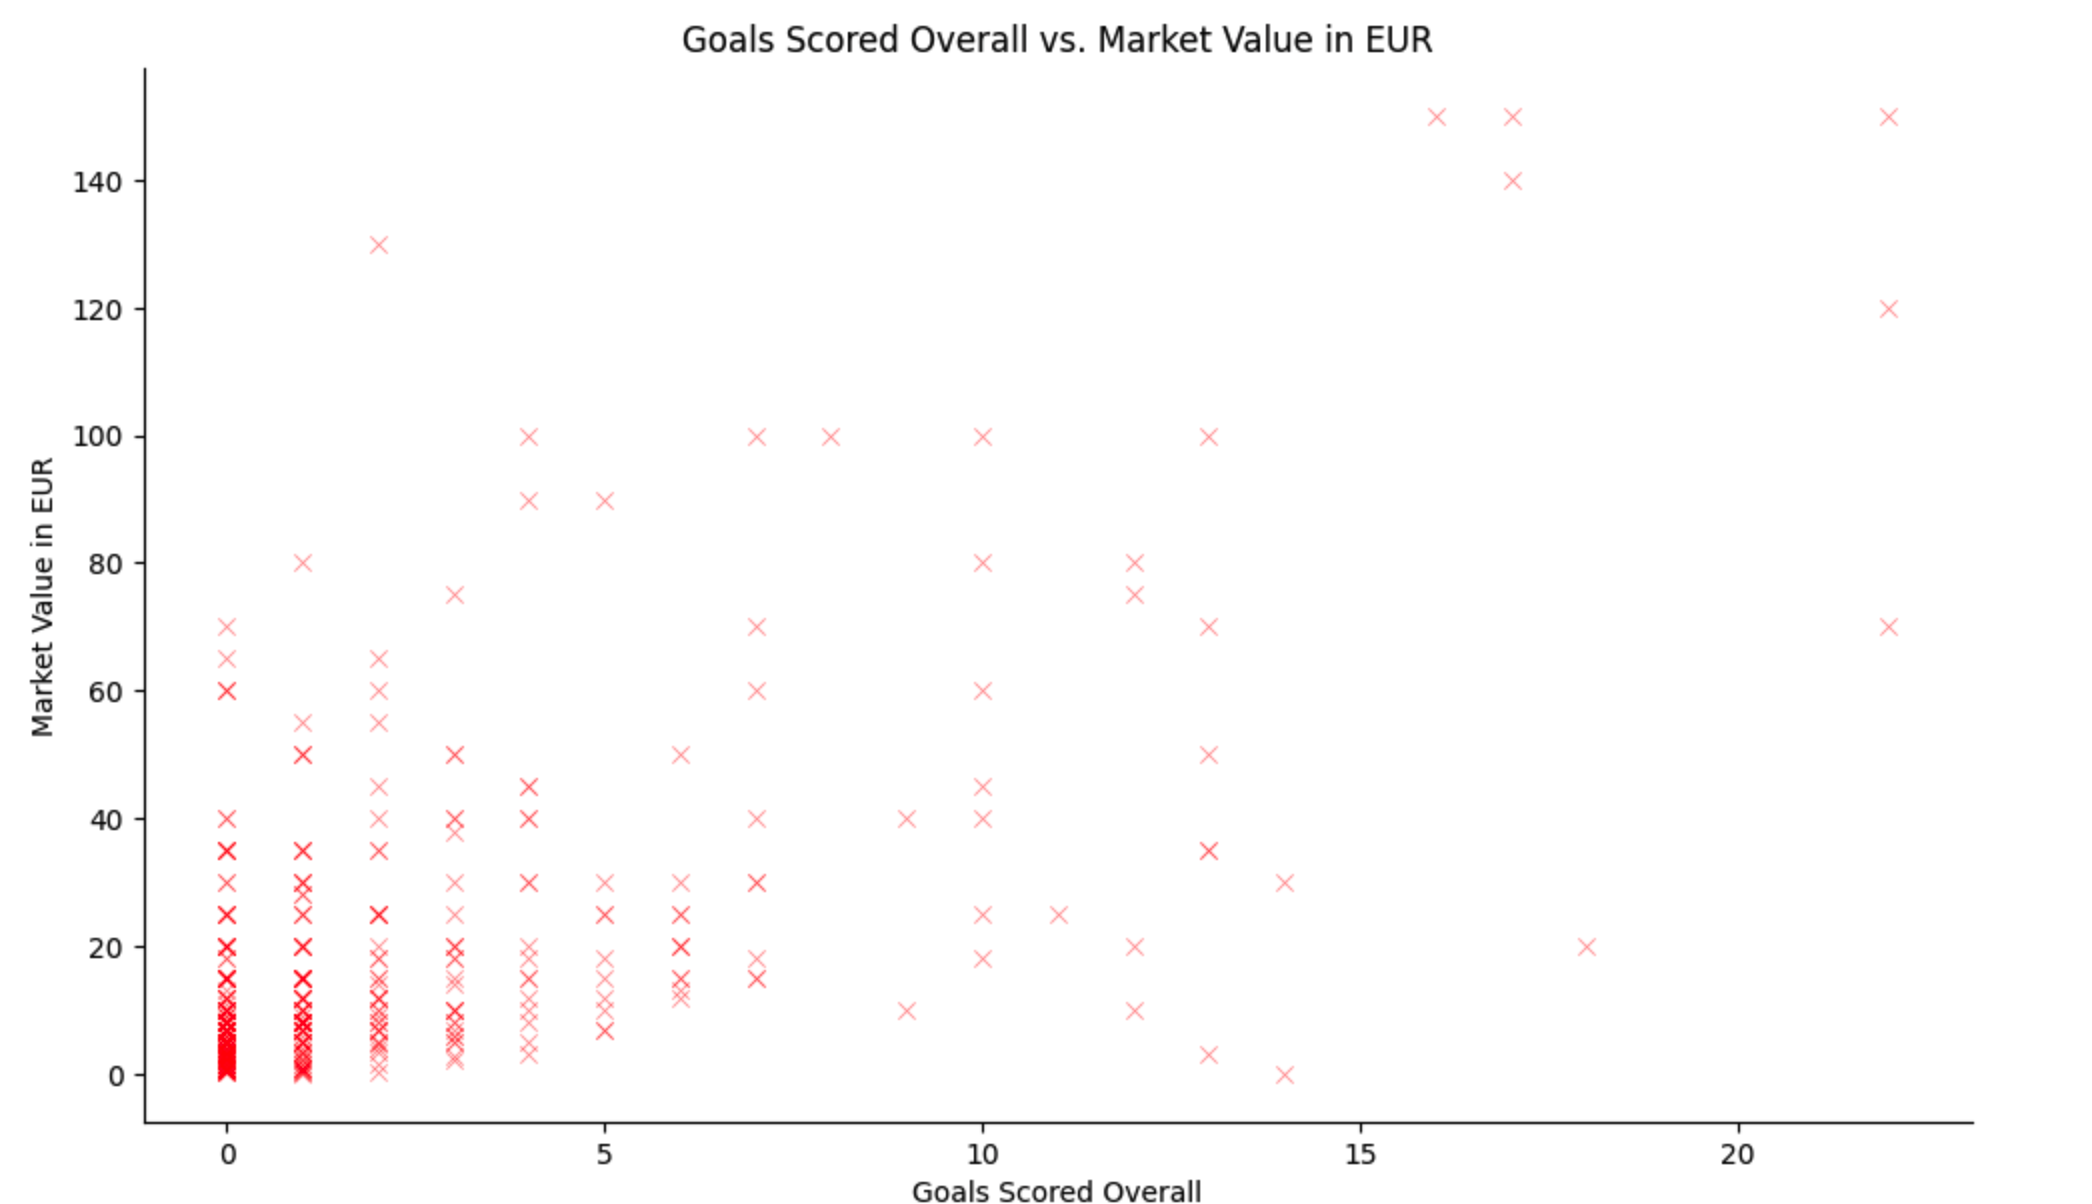
\includegraphics[width=\linewidth]{goals.png} 
        \label{fig:zdjecie}
    \end{minipage}
    \hfill 
\end{figure}


\begin{figure}[H]
    \centering
        \begin{minipage}{0.5\textwidth} 
        \centering Zależność ceny od asyst :
    \end{minipage}
    \begin{minipage}{1\textwidth} 
        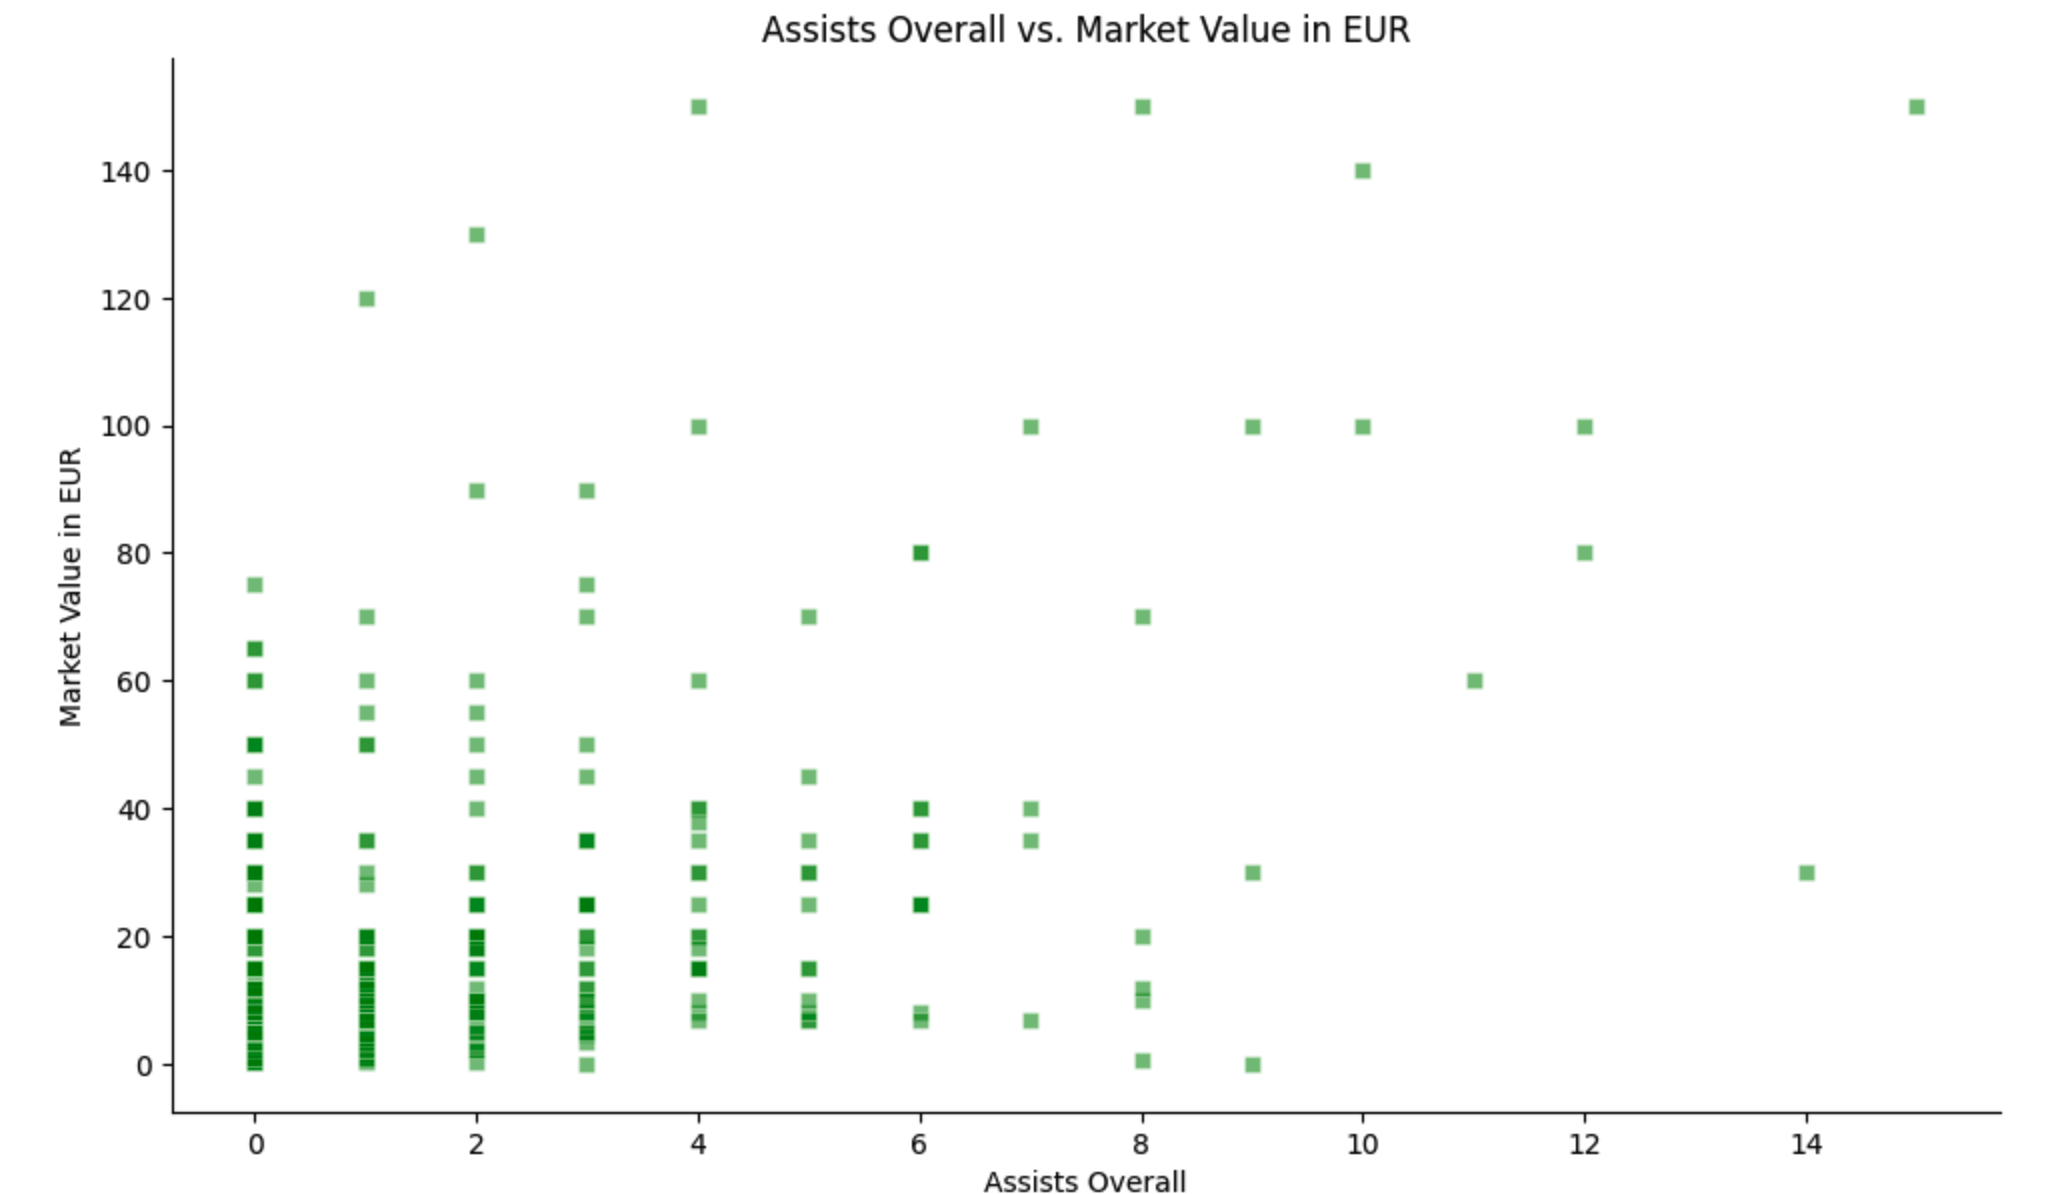
\includegraphics[width=\linewidth]{assists.png} 
        \label{fig:zdjecie}
    \end{minipage}
    \hfill 

\end{figure}


\begin{figure}[H]
    \centering
        \begin{minipage}{0.5\textwidth} 
        \centering Zależność ceny od wieku :
    \end{minipage}
    \begin{minipage}{1\textwidth} 
        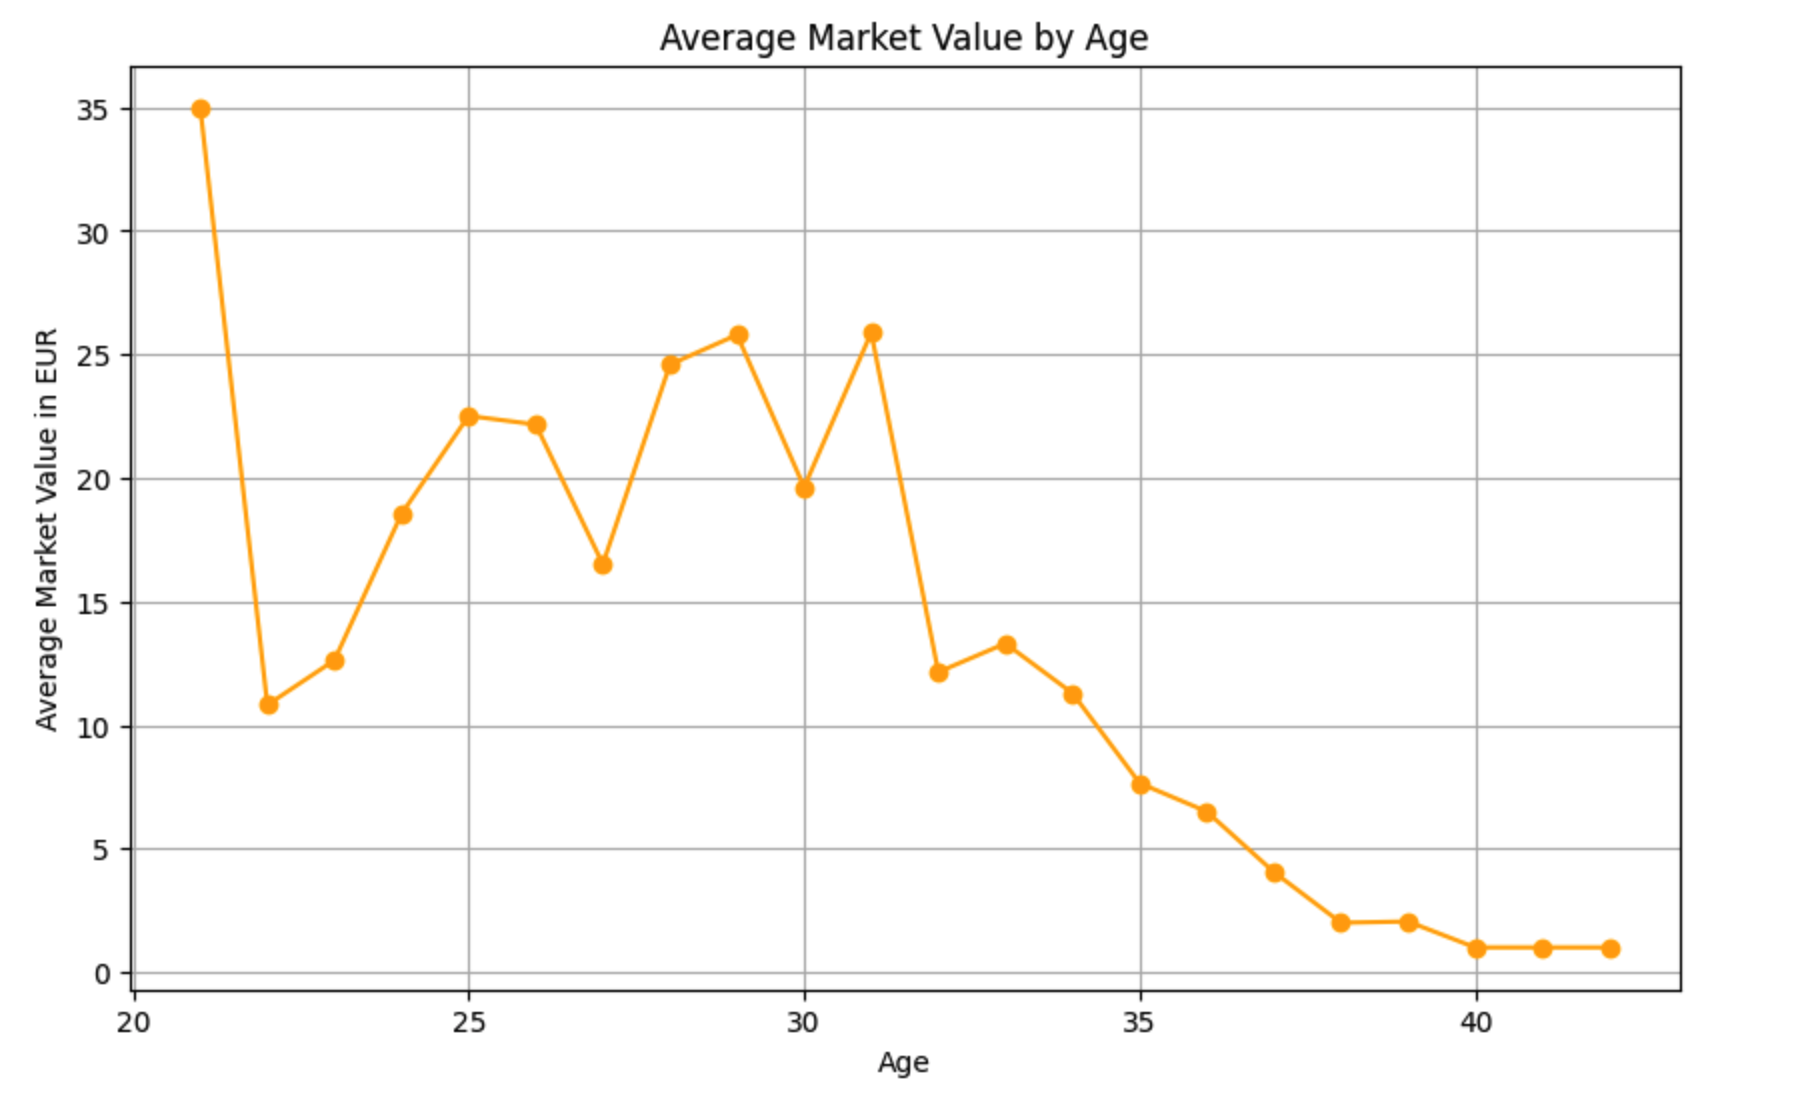
\includegraphics[width=\linewidth]{age.png} 
        \label{fig:zdjecie}
    \end{minipage}
    \hfill 

\end{figure}

\begin{figure}[H]
    \centering
        \begin{minipage}{0.5\textwidth} 
        \centering Zależność ceny od pozycji :
    \end{minipage}
    \begin{minipage}{1\textwidth} 
        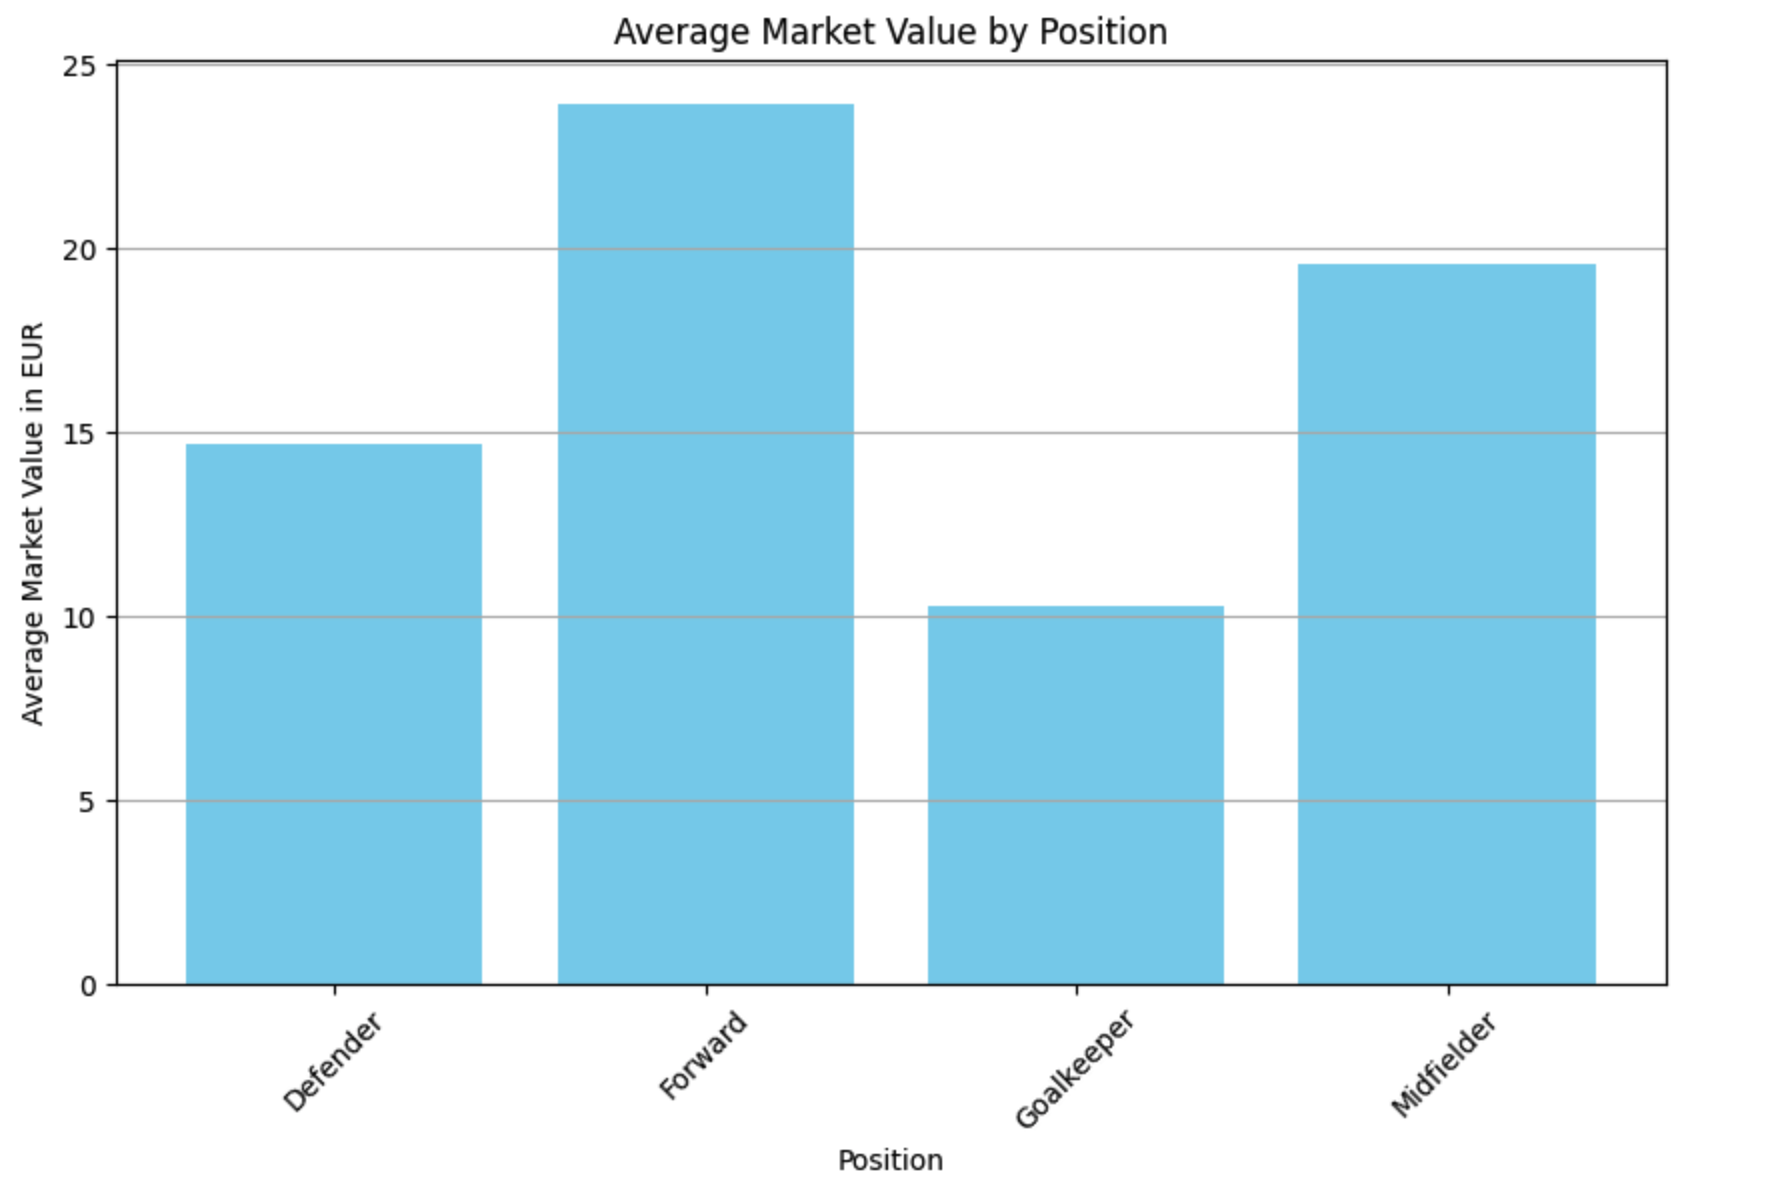
\includegraphics[width=\linewidth]{position.png} 
        \label{fig:zdjecie}
    \end{minipage}
    \hfill 

\end{figure}

\begin{figure}[H]
    \centering
        \begin{minipage}{0.5\textwidth} 
        \centering Zależność ceny od kraju pochodzenia :
    \end{minipage}
    \begin{minipage}{1\textwidth} 
        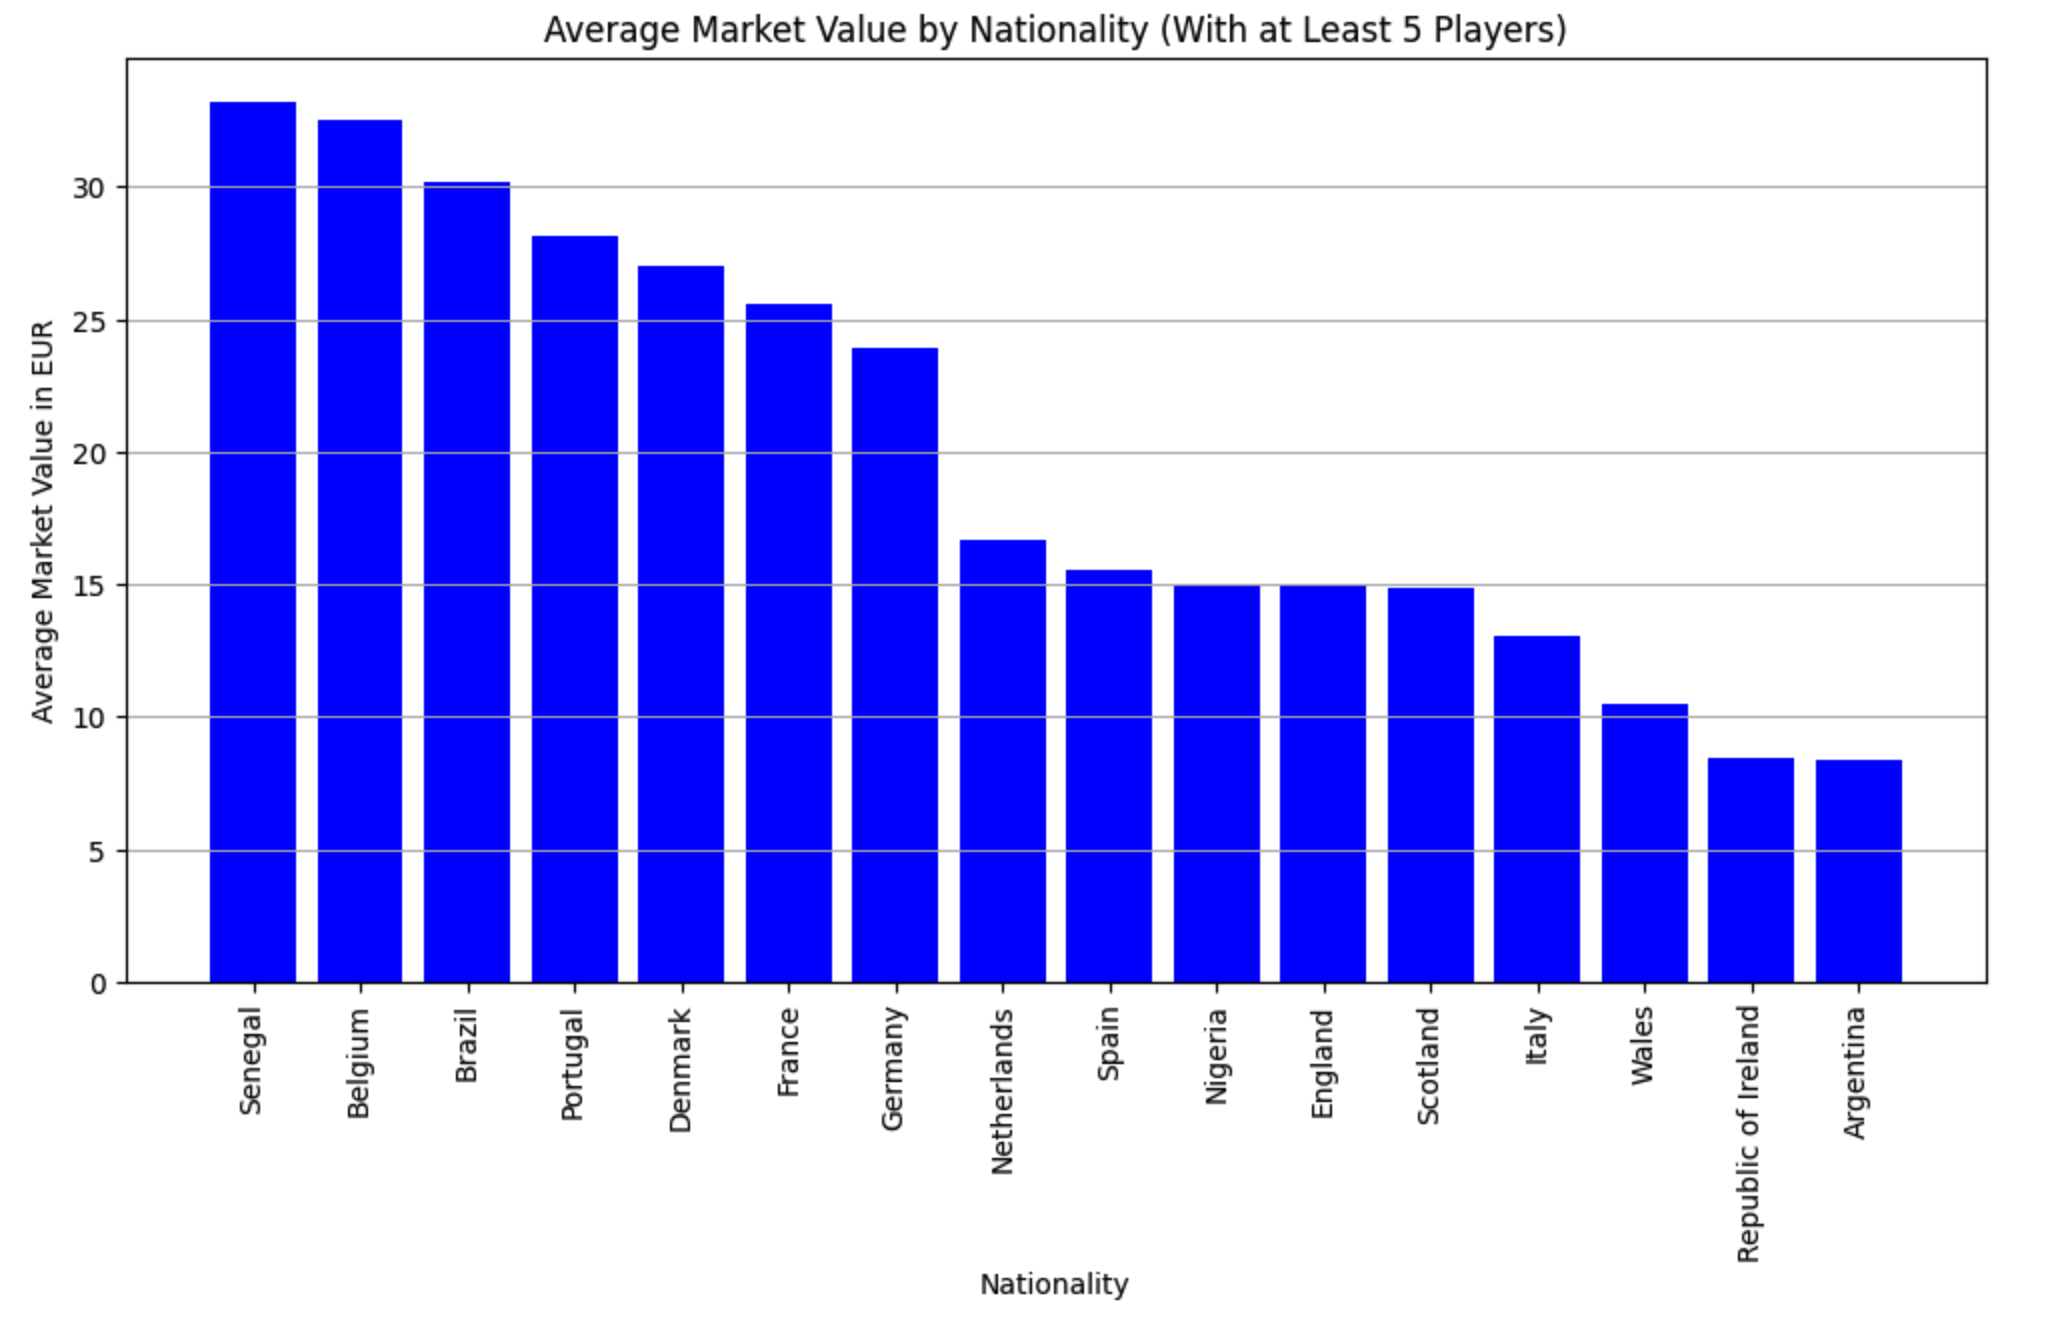
\includegraphics[width=\linewidth]{nationality.png} 
        \label{fig:zdjecie}
    \end{minipage}
    \hfill 

\end{figure}

\begin{figure}[H]
    \centering
        \begin{minipage}{0.5\textwidth} 
        \centering Zależność średniej ceny zawodnika klubu od liczby punktów w lidze :
    \end{minipage}
    \begin{minipage}{1\textwidth} 
        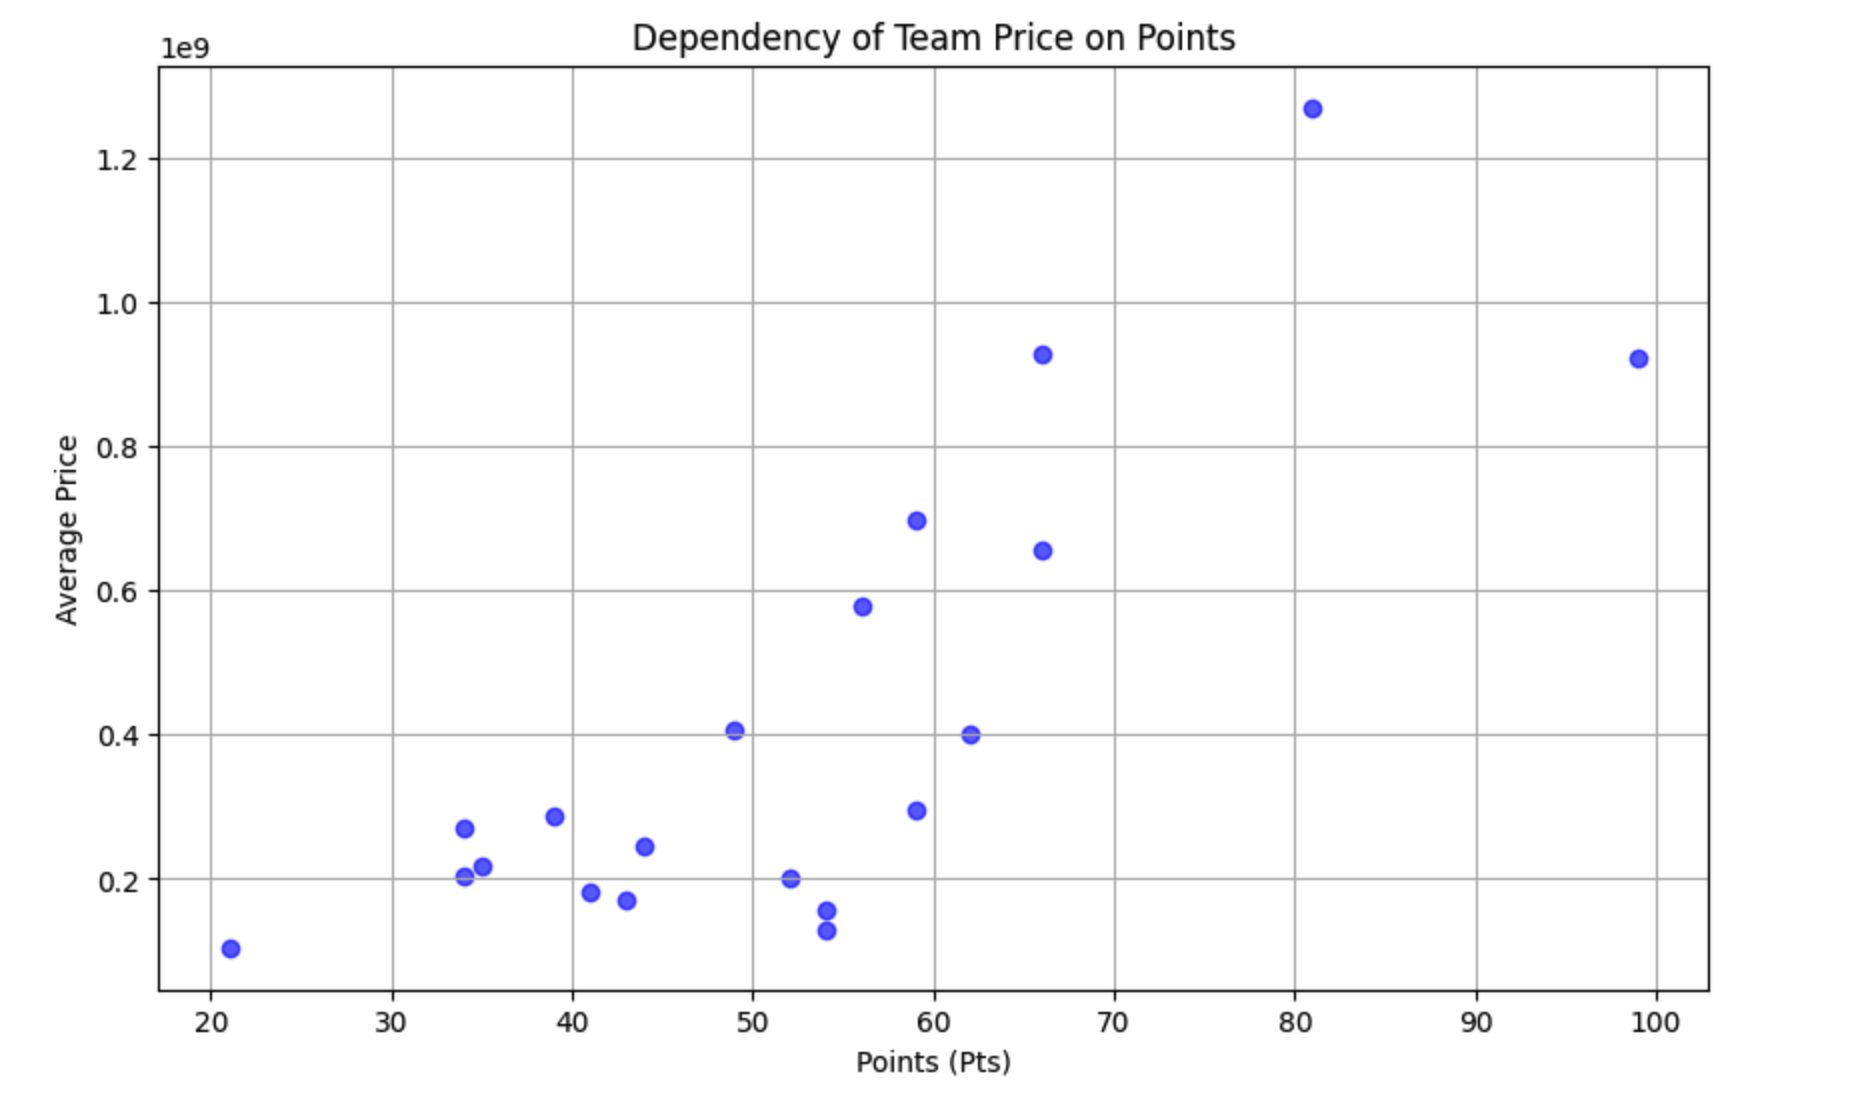
\includegraphics[width=\linewidth]{price.png} 
        \label{fig:zdjecie}
    \end{minipage}
    \hfill 

\end{figure}

\textbf{Wyszukiwanie zależnośći}


1) Zależność ceny od minut zagranych w sezonie: Na podstawie danych wykresu, wydaje się, że cena zawodnika rośnie wraz z ilością minut spędzonych na boisku. Możemy przypuszczać, że kluby skupiają się na zawodnikach, którzy mają dużą liczbę minut gry.

2) Zależność ceny od strzelonych bramek: Istnieje widoczna tendencja wzrostowa między ceną zawodnika a liczbą bramek, co sugeruje, że zawodnicy, którzy zdobywają więcej goli, są bardziej pożądani na rynku.

3) Zależność ceny od asyst: Wydaje się, że liczba asyst również wpływa na cenę zawodnika, choć nie tak wyraźnie jak liczba bramek. Zawodnicy, którzy potrafią doskonale współpracować z innymi, mogą być wyceniani wyżej.

4) Zależność ceny od wieku: Istnieje pewna zależność między wiekiem a ceną, gdzie młodsi zawodnicy mogą być wyceniani wyżej ze względu na swoją perspektywę rozwoju, podczas gdy starsi zawodnicy mogą być mniej atrakcyjni ze względu na potencjalny spadek wydajności.

5) Zależność ceny od pozycji: Ceny zawodników mogą się różnić w zależności od ich pozycji na boisku. Na przykład, napastnicy mogą być wyceniani wyżej niż obrońcy ze względu na ich umiejętność zdobywania bramek.

6) Zależność ceny od kraju pochodzenia: Cena zawodnika może być również uzależniona od jego kraju pochodzenia, gdzie zawodnicy z bardziej konkurencyjnych lig lub popularnych krajów mogą być wyceniani wyżej.

7) Zależność średniej ceny zawodnika klubu od liczby punktów w lidze: Możemy zauważyć, że kluby z większą liczbą punktów w lidze mogą mieć droższych zawodnikówśś

\section{Tworzenie modeli}

\subsection{Przygotowywanie danych}
Dla używania zależności kraju pochodzenia i pozycji od cena, należało zamienic tekst (String) na liczbę odpowiadające każdemu kraju/pozycji.
\subsection{Podział danych}
Dane zostały podzielone na treningowe oraz testowe za pomocą funkcji w bibliotece sklearn.
\subsection{Dane do przeanalizowania}
Po przeprowadzeniu różnych prób, najlepsze wyniki uzyskano z modelami uwzględniającymi następujące cechy:
\begin{itemize}
    \item Wiek
    \item Pozycja
    \item Liczba zagranych minut
    \item Kraj pochodzenia
    \item Liczba bramek
    \item Liczba asyst
    \item Liczba punktów drużyny
    \item Cena drużyny
\end{itemize}

\subsection{Tworzenia modeli przewidywających}
Na podstawie zbiorów naszych danych były trenowane 4 modele :
\begin{itemize}
    \item Regresja Liniowa
    \item Maszyna wektorów nośnych (SVM with Standart Scaler)
    \item Metoda Lasu Losowego (Random Forest)
    \item Uogólniony model liniowy (GLM)
\end{itemize}
Po przetrenowaniu i przewydywaniu mamy następną sytuację:
\begin{figure}[H] 
    \centering
    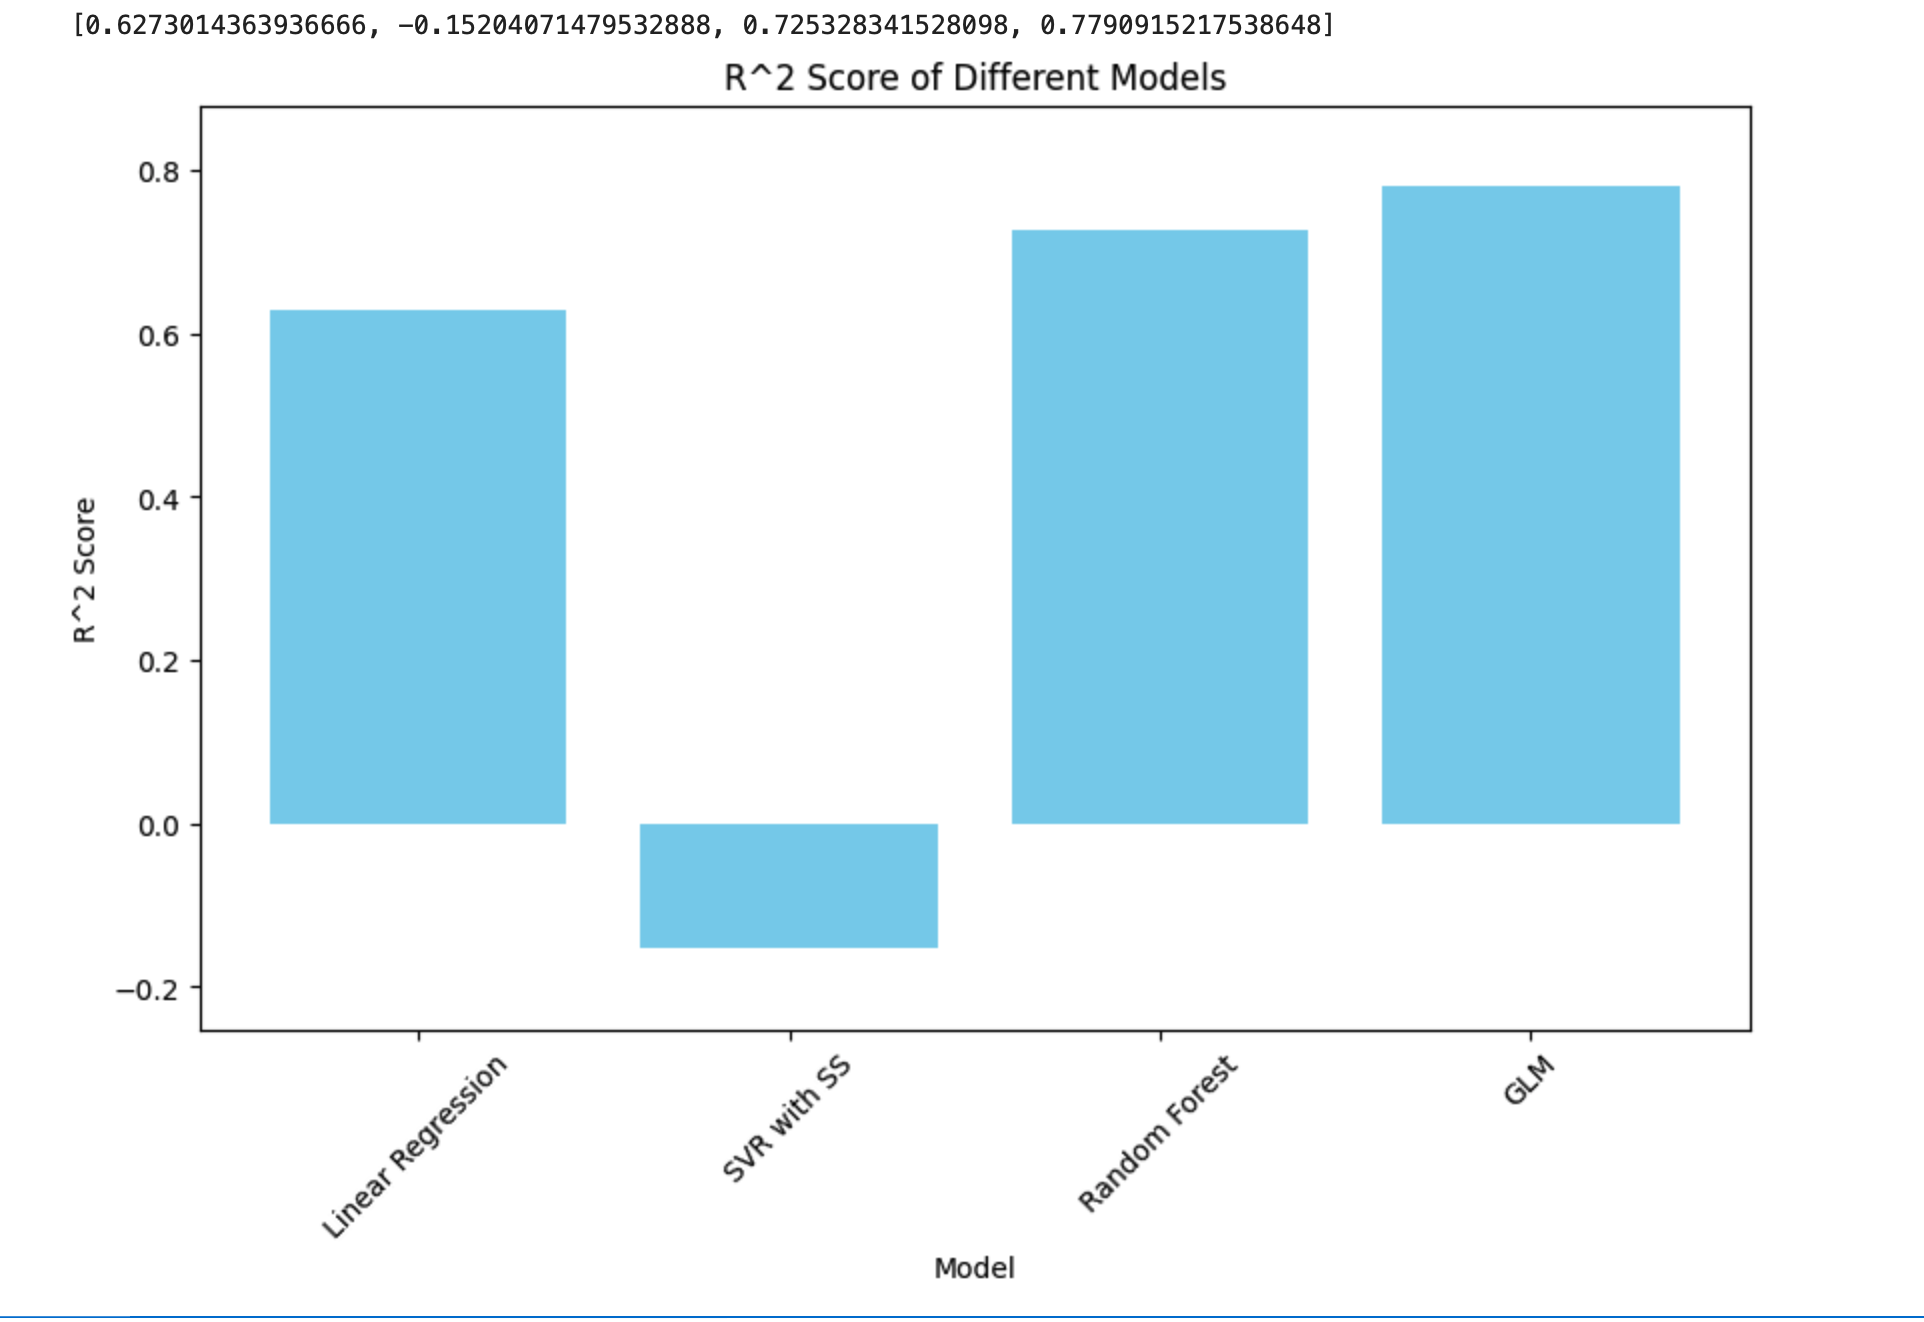
\includegraphics[width=\textwidth]{Machines.png}
    
\end{figure}

Współczynnik determinacji \( R^2 \) jest miarą, która wskazuje, jak dobrze model regresyjny wyjaśnia zmienność danych. Jego wartość wynosi od 0 do 1:

\begin{itemize}
    \item \textbf{\( R^2 = 1 \)}: Model idealnie wyjaśnia zmienność danych.
    \item \textbf{\( R^2 = 0 \)}: Model nie wyjaśnia żadnej zmienności danych.
    \item \textbf{Im bliżej 1, tym lepsze dopasowanie modelu do danych.}
    \item \textbf{Im bliżej 0, tym gorsze dopasowanie modelu do danych.}
\end{itemize}


\textbf{Jak można zauważyć, model maszyny wektorów nośnych (SVM) nie jest efektywny w naszym przypadku.}

Dla analizy skuteczności modeli można dodać Średni błąd bezwzględny (MAE), Średni błąd kwadratowy (MSE) oraz Pierwiastek średniokwadratowy błędu (RMSE).

Po dodaniu tych atrybutów do naszego \( R^2 \)
  i usunięciu z analizy \textbf{maszyny wektorów nośnych}, mamy:

\begin{figure}[H]
    \centering
    \begin{minipage}{0.3\textwidth}
        \centering
        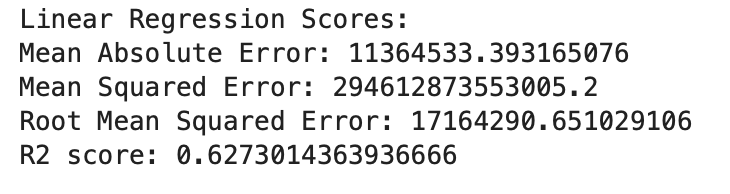
\includegraphics[width=\linewidth]{LReg.png}
    \end{minipage}
    \hfill
    \begin{minipage}{0.3\textwidth}
        \centering
        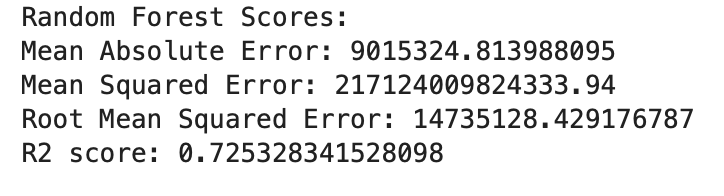
\includegraphics[width=\linewidth]{RF.png}
    \end{minipage}
    \hfill
    \begin{minipage}{0.3\textwidth}
        \centering
        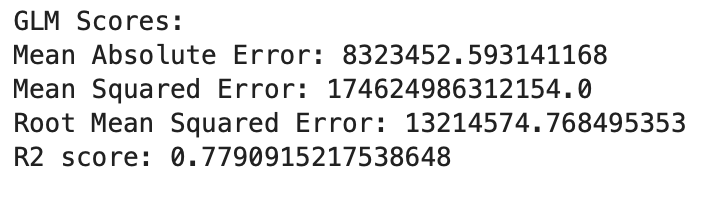
\includegraphics[width=\linewidth]{GLM.png}

    \end{minipage}
\end{figure}

Widać, że najefektywniejszym modelem przewidywającym jest \textbf{uogólniony model liniowy (GLM)}

\section{Wnioski}
Analiza i przewidywanie cen zawodników na podstawie różnych zbiorów danych wykazała, że model \textbf{GLM} jest najbardziej efektywny w tym zadaniu. Zostało to potwierdzone porównaniem wyników MAE, MSE, RMSE oraz \( R^2 \)
  z innymi modelami. Pobieranie danych z różnych źródeł i ich powiązanie między sobą dało możliwość zaprojektowania bardziej dokładnego modelu.
\section{Źródła}
\begin{flushleft}
    \href{https://www.kaggle.com/datasets/davidcariboo/player-scores/data}{https://www.kaggle.com/datasets/davidcariboo/player-scores/data}

    \href{https://www.kaggle.com/code/davidcoxon/football-transfer-market-eda-basic-modelling}{https://www.kaggle.com/code/davidcoxon/football-transfer-market-eda-basic-modelling}

    \href{https://www.eurosport.com/football/premier-league/2019-2020/standings.shtml}{https://www.eurosport.com/football/premier-league/2019-2020/standings.shtml}

    \href{https://footystats.org/download-stats-csv}{https://footystats.org/download-stats-csv}
\end{flushleft}

  
\end{document}

